\documentclass[12pt]{article}

\setlength\parindent{0pt}
\newcommand{\myt}[1]{\textbf{\underline{#1}}}

\usepackage{mathtools}
\usepackage{amssymb}
\usepackage{tikz,ifthen,amsmath,amssymb,fancyhdr,comment,lastpage}
%\usetikzlibrary{shapes,chains,positioning}

\title{\vspace{-15ex}CS 241 Lec 8\vspace{-1ex}}
\date{June 1st, 2015}
\author{Graham Cooper}

\begin{document}
	\maketitle
	
	\section*{Linker Algorithm}
	
	Input: MERL files m1 and m2\\
	Output: Single MERL file with m2 linked after m1\\
	
	$\alpha \leftarrow$ m1.codeLen - 12\\
	relocate m2.code by $\alpha$\\
	add $\alpha$ to every address in m2.symtbl\\
	if m1.exports.labels $\cap$ m2.exports.labels $\neq \emptyset$, ERROR \\
	for each \textless addr$_1$, label\textgreater $\in$ m1.imports\\
	-- if $\exists$\textless addr$_2$, label\textgreater $\in$ m2.exports\\
	---- m1.code[addr$_1$] $\leftarrow$ addr$_2$\\
	---- remove \textless addr$_1$, label \textgreater from m1.imports\\
	---- add addr$_1$ to m1.relocates\\
	for each \textless addr$_2$, label \textgreater $\in$ m2.imports \\
	-- if $\exists$ \textless addr$_1$, label \textgreater $\in$ m1.imports\\
	---- m2.code[addr$_2$] $\leftarrow$ addr$_1$\\
	---- remove \textless addr$_2$, label \textgreater from m2.imports\\
	---- add addr$_2$ to m2.relocates\\
	imports = m1.imports $\cup$ m2.imports\\
	exports = m1.exports $\cup$ m2.exports\\
	relocates = m1.relocates $\cup$ m2.relocates\\
	output MERL cookie\\
	output total codeLen + total(import,exports,relocates) + 12\\
	output total codLen + 12\\
	output m1.code\\
	output m2.code\\
	output imports, exports, relocates\\
	
	\section*{Formal Languages}
	
	High level language $\rightarrow$ Compiler $\rightarrow$ Assembly Language\\
	\subsection*{Assembly:}
	- simple structure\\
	- easy to recognize\\
	- straightforward, unambiguous translation to machine code\\
	
	\subsection*{High-level}
	- more complex structure \\
	- harder to recognize\\
	- no single translation to machine code\\
	
	\subsection*{How can we handle the complexity of a compiler?}
	
	Start with a formal theory of string recognition\\
	- general principals that work for any programming language\\
	
	\subsubsection*{Definitions}
	Alphabet: 
	\begin{itemize}
		\item Finite set of symbols (eg. \{a,b,c\})
		\item typically denoted $\Sigma$, as in $\Sigma$ = \{a,b,c\}
	\end{itemize}
	
	string(or word):
	\begin{itemize}
		\item finite sequence of symbols (from $\Sigma$)
		\item eg. a, aba, cbca, ...
		\item length of a word $|\omega|$ = number of characters in the word,
		\item eg. $|aba|$ = 3
		\item empty string - an empty sequence of symbols use $\epsilon$ to denote the empty string. $\epsilon$ is not a symbol, $|\epsilon|$ = 0
	\end{itemize}
	
	Language:
	\begin{itemize}
		\item a set of strings (words)
		\item eg $\{a^{2n}b | n \geq 0\}$ all words with an even number of a's followed by b
		\item NOTE: $\epsilon$ vs \{\}, epsilon is the empty word, but the empty braces is the empty language (contains no words). \{$\epsilon\}$ is a singleton language, that contains only $\epsilon$
	\end{itemize}
	
	\subsection*{Our task}
	Question: How can we recognize automatically whether a given string belongs to a given language?\\
	
	Answer: Depends on how complex the language is.\\
	\begin{itemize}
		\item $\{a^2n b | n \geq 0\}$ - easy
		\item \{valid MIPS assembly programs\} - almost as easy
		\item \{valid Java Programs\} - harder
		\item some languages - impossible
	\end{itemize}
	
	Characterize languages according to how difficult the recognition process is. - classes of languages based on "hardness"\\
	\begin{itemize}
		\item finite
		\item regular
		\item context-free
		\item context-sensitive
		\item recursive languages
		\item etc.
	\end{itemize}
	Top is easy, bottom is impossible\\
	
	Want to work at as easy a level as possible, move to a harder level if neccessary.\\
	
	Finite Languages:
	\begin{itemize}
		\item have finitely many words
		\item can recognize a word by comparing with every lement of the set (finite!)
		\item can we do this efficiently?
	\end{itemize}
	
	Exercise: L = \{cat, car, cow\}\\
	Write code to answer $\omega \in L$ such that $\omega$ is scanned exactly once, without storing previously-seen chars.\\
	
	Scan input left to right\\
	if first character is c, move on, else error\\
	if next character is a: \\
	-- if next char is t : \\
	---- if input is empty, accept, else error\\
	-- else if char is r: \\
	---- if input is empty, accept, else error \\
	-- else error
	else if character is o : \\
	-- if next character is w :
	---- if input is empty, accept, else error \\
	-- else error\\
	else error\\
	
	\begin{center}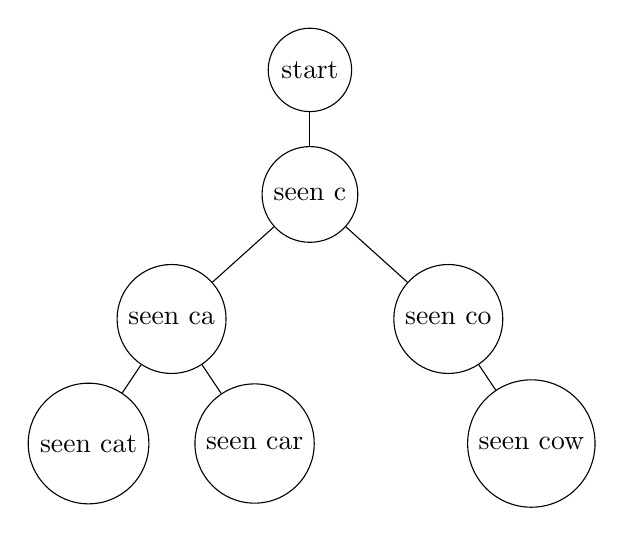
\begin{tikzpicture}[
		level distance=45 pt,
		every node/.style={circle,draw},
		level 1/.style={sibling distance=200 pt},
		level 2/.style={sibling distance=100 pt},
		level 3/.style={sibling distance=60 pt}
		]
		\node {start}
		child {node {seen c}
			child {node {seen ca}
				child {node {seen cat}}
				child {node {seen car}}
			}
			child {node {seen co}
				child [missing]
				child {node {seen cow}}
			}
		};
		child [missing]
		\end{tikzpicture}\end{center}
	
	Bubbles are states, configurations f the program based on the input seen. The leaf nodes mean you accept if you stop there.\\
	
	Since programming languages don't usually admit only finitely many programs, finite languages not that useful.\\
\end{document}
